\tikzset{every picture/.style={line width=0.75pt}} %set default line width to 0.75pt        

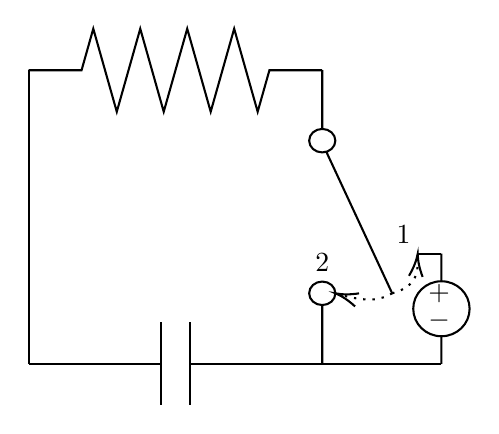
\begin{tikzpicture}[x=0.75pt,y=0.75pt,yscale=-1,xscale=1]
%uncomment if require: \path (0,504); %set diagram left start at 0, and has height of 504

%Shape: Resistor [id:dp30608216087842166] 
\draw   (150,80.58) -- (175.46,80.58) -- (181.11,60.58) -- (192.43,100.58) -- (203.74,60.58) -- (215.05,100.58) -- (226.37,60.58) -- (237.68,100.58) -- (248.99,60.58) -- (260.31,100.58) -- (265.97,80.58) -- (291.42,80.58) ;
%Straight Lines [id:da858527027889131] 
\draw    (150,80.58) -- (150,222) ;
%Shape: Capacitor [id:dp9610189215282299] 
\draw   (150,222) -- (213.64,222) (227.78,202) -- (227.78,242) (213.64,202) -- (213.64,242) (227.78,222) -- (291.42,222) ;
%Shape: Simple Switch [id:dp8738783462574553] 
\draw   (291.42,80.58) -- (291.42,108.86) (291.42,193.72) -- (291.42,222) (293.53,120.18) -- (325.11,188.06) (291.42,182.4) .. controls (294.91,182.4) and (297.74,184.93) .. (297.74,188.06) .. controls (297.74,191.18) and (294.91,193.72) .. (291.42,193.72) .. controls (287.93,193.72) and (285.11,191.18) .. (285.11,188.06) .. controls (285.11,184.93) and (287.93,182.4) .. (291.42,182.4) -- cycle (291.42,108.86) .. controls (294.91,108.86) and (297.74,111.4) .. (297.74,114.52) .. controls (297.74,117.64) and (294.91,120.18) .. (291.42,120.18) .. controls (287.93,120.18) and (285.11,117.64) .. (285.11,114.52) .. controls (285.11,111.4) and (287.93,108.86) .. (291.42,108.86) -- cycle ;
%Straight Lines [id:da2492031249151494] 
\draw    (348.84,222) -- (291.42,222) ;
%Shape: Output [id:dp8123576692630616] 
\draw   (348.84,182.25) .. controls (356.34,182.25) and (362.42,188.18) .. (362.42,195.5) .. controls (362.42,202.82) and (356.34,208.75) .. (348.84,208.75) .. controls (341.34,208.75) and (335.26,202.82) .. (335.26,195.5) .. controls (335.26,188.18) and (341.34,182.25) .. (348.84,182.25) -- cycle (348.84,169) -- (348.84,182.25) (348.84,222) -- (348.84,208.75) ;
%Straight Lines [id:da24217538064489208] 
\draw    (348.84,169) -- (337.42,169) ;
%Curve Lines [id:da8139879269218222] 
\draw  [dash pattern={on 0.84pt off 2.51pt}]  (325.11,188.06) .. controls (338.21,184.49) and (337.46,176.31) .. (337.38,171) ;
\draw [shift={(337.42,169)}, rotate = 94.82] [color={rgb, 255:red, 0; green, 0; blue, 0 }  ][line width=0.75]    (10.93,-3.29) .. controls (6.95,-1.4) and (3.31,-0.3) .. (0,0) .. controls (3.31,0.3) and (6.95,1.4) .. (10.93,3.29)   ;
%Curve Lines [id:da1445503769752734] 
\draw  [dash pattern={on 0.84pt off 2.51pt}]  (325.11,188.06) .. controls (320.2,190.88) and (314.48,192.84) .. (299.64,188.62) ;
\draw [shift={(297.74,188.06)}, rotate = 16.9] [color={rgb, 255:red, 0; green, 0; blue, 0 }  ][line width=0.75]    (10.93,-3.29) .. controls (6.95,-1.4) and (3.31,-0.3) .. (0,0) .. controls (3.31,0.3) and (6.95,1.4) .. (10.93,3.29)   ;

% Text Node
\draw (335.42,165.6) node [anchor=south east] [inner sep=0.75pt]    {$1$};
% Text Node
\draw (291.42,179) node [anchor=south] [inner sep=0.75pt]    {$2$};
% Text Node
\draw (341,182.4) node [anchor=north west][inner sep=0.75pt]    {$+$};
% Text Node
\draw (341,195.4) node [anchor=north west][inner sep=0.75pt]    {$-$};


\end{tikzpicture}
